% =====================================================================
\chapter{Um toque de Cálculo}\label{cap:11}
\naaula{41 a 45}

Você não precisa ter estudado Cálculo para acompanhar este capítulo. Vamos usar uma única ideia —
a \textbf{derivada} — e uma única regra para calculá-la. Com elas, dá para medir quanto um custo
cresce a cada elemento a mais e até descobrir o melhor valor de um parâmetro de um algoritmo.

\section{Derivada: a inclinação de uma curva}

Nos capítulos anteriores, comparamos funções pelo \enquote{quanto crescem}. A derivada torna isso
preciso: ela mede \textbf{a taxa de crescimento} de uma função em cada ponto — quanto a saída
aumenta quando a entrada aumenta um pouquinho.

Graficamente, a derivada de $T$ no ponto $n$ é a \textbf{inclinação da reta tangente} (a reta que
só \enquote{encosta} na curva naquele ponto). Uma inclinação 4 quer dizer: perto daquele ponto,
cada unidade a mais em $n$ aumenta $T$ em cerca de 4.

\begin{figure}[!htb]
  \centering
  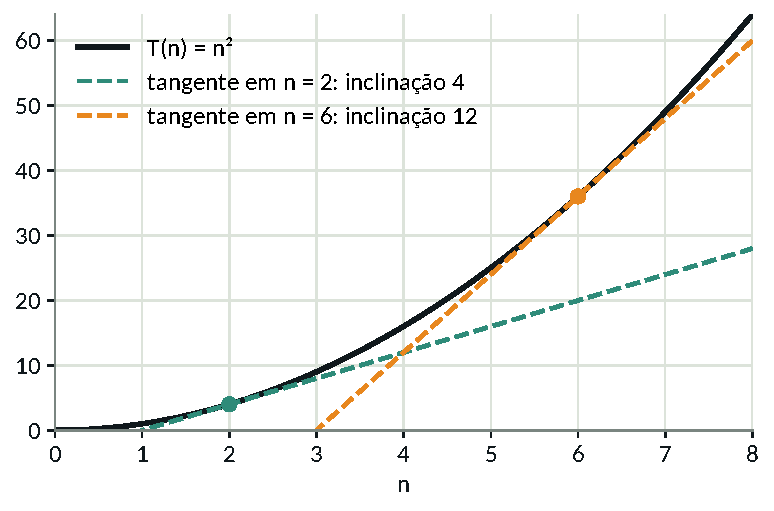
\includegraphics[width=0.72\textwidth]{figuras/f11_tangentes.pdf}
  \caption{Em $T(n) = n^2$, a tangente em $n = 2$ tem inclinação 4; em $n = 6$, inclinação 12.
  Quanto mais à direita, mais íngreme: o crescimento acelera.}
\end{figure}

Escrevemos a derivada de $T(n)$ como $T'(n)$ (lê-se \enquote{tê linha de ene}). Se $T'(n)$ é
constante, a função cresce sempre no mesmo ritmo (é linear); se $T'(n)$ aumenta com $n$, o
crescimento acelera.

\section{A regra da potência}

Para as funções que aparecem em análise de algoritmos, uma regra resolve quase tudo:

\begin{center}
\colorbox{edtealclaro}{\large\quad $\dfrac{d}{dn}\left(n^p\right) = p \cdot n^{p-1}$\quad}
\qquad \small (\enquote{o expoente desce multiplicando e diminui 1})
\end{center}

\begin{center}
\begin{tabularx}{\textwidth}{P{3.4cm} P{3.6cm} L}
\cab \tc{Função} & \tc{Derivada} & \tc{Como} \\
$n$ & $1$ & $n = n^1 \to 1 \cdot n^0 = 1$ \\
\rowcolor{edfundo} $n^2$ & $2n$ & $2 \cdot n^1$ \\
$n^3$ & $3n^2$ & $3 \cdot n^2$ \\
\rowcolor{edfundo} $\sqrt{n} = n^{1/2}$ & $\dfrac{1}{2\sqrt{n}}$ & $\tfrac{1}{2} \cdot n^{-1/2}$ \\
$\dfrac{1}{n} = n^{-1}$ & $-\dfrac{1}{n^2}$ & $-1 \cdot n^{-2}$ \\
\rowcolor{edfundo} uma constante, como $7$ & $0$ & constantes não variam \\
\end{tabularx}
\end{center}

Duas regras completam o kit: a derivada de uma \textbf{soma} é a soma das derivadas, e uma
\textbf{constante multiplicando} continua multiplicando. Por exemplo:
$\dfrac{d}{dn}\left(3n^2 + 5n + 2\right) = 3 \cdot 2n + 5 \cdot 1 + 0 = 6n + 5$.

\subsection{A regra da cadeia para \texorpdfstring{$u^p$}{u elevado a p}}

Quando o que está elevado a $p$ não é o próprio $n$, mas uma expressão $u$ que depende de $n$,
multiplicamos também pela derivada de $u$:
\[
\frac{d}{dn}\left(u^p\right) = p \cdot u^{p-1} \cdot u'
\]
Exemplos: $\dfrac{d}{dn}(n + 1)^2 = 2(n + 1) \cdot 1 = 2n + 2$ \quad e \quad
$\dfrac{d}{dn}(3n - 2)^2 = 2(3n - 2) \cdot 3 = 18n - 12$.

\section{Custo marginal: quanto custa um elemento a mais?}

A derivada responde a uma pergunta prática: \textbf{se o problema ganhar um elemento, quanto
trabalho a mais o algoritmo terá?}

No pior caso do Insertion Sort, $T(n) = \dfrac{n(n-1)}{2} = \dfrac{n^2}{2} - \dfrac{n}{2}$.
Pela regra da potência:
\[
T'(n) = \frac{2n}{2} - \frac{1}{2} = n - \frac{1}{2} \approx n.
\]
Cada elemento a mais custa cerca de $n$ comparações extras. Conferindo com a conta exata:
$T(n + 1) - T(n) = \dfrac{(n+1)n}{2} - \dfrac{n(n-1)}{2} = n$. Para um vetor de 1.000 elementos,
acrescentar mais um custa cerca de 1.000 comparações; para 1.000.000 de elementos, cerca de um
milhão.

Compare com a busca linear, $T(n) = n$: $T'(n) = 1$. Cada elemento a mais custa sempre a mesma
coisa, uma comparação. \textbf{Derivada constante significa crescimento linear; derivada que
cresce significa crescimento acelerado.}

\section{Achando o melhor parâmetro: a busca por saltos}

Agora um problema em que a derivada \emph{resolve} uma questão de projeto.

Queremos procurar um valor num vetor \textbf{ordenado} com $n$ elementos — por exemplo, uma
lista de chamada com 10.000 nomes em ordem alfabética. A busca linear faria até 10.000
comparações. A \textbf{busca por saltos} aproveita a ordem e o acesso por índice em $O(1)$ da
lista contígua (Aula 1):

\begin{enumerate}
  \item Salte de $m$ em $m$ posições, olhando só o último elemento de cada bloco, até achar um
        bloco cujo último elemento seja maior ou igual ao valor procurado.
  \item Faça uma busca linear só dentro desse bloco.
\end{enumerate}

\begin{figure}[!htb]
\centering
\begin{tikzpicture}[scale=0.42]
  \foreach \i in {0,...,23} \draw[fill=white, draw=edcinzaclaro, line width=0.7pt] (\i, 0) rectangle ++(0.9, 0.9);
  \foreach \b in {3,7,11,15} \draw[fill=edtealclaro, draw=edteal, line width=0.9pt] (\b, 0) rectangle ++(0.9, 0.9);
  \foreach \i in {16,...,19} \draw[fill=edlaranjaclaro, draw=edlaranja, line width=0.9pt] (\i, 0) rectangle ++(0.9, 0.9);
  \foreach \a/\b in {-1/3, 3/7, 7/11, 11/15, 15/19}
    \draw[-{Latex}, edteal, line width=1pt] (\a+0.45, 1.1) to[bend left=40] (\b+0.45, 1.1);
  \node[font=\small, color=edteal, anchor=south] at (8, 2.4) {fase 1: saltos de $m = 4$ posições};
  \node[font=\small, color=edlaranja, anchor=north] at (17.9, -0.3) {fase 2: busca linear no bloco};
\end{tikzpicture}
\caption{Busca por saltos com $m = 4$: os saltos examinam o fim de cada bloco (verde); o valor
está no bloco laranja, percorrido um a um.}
\end{figure}

Qual o melhor tamanho de salto $m$? Se $m$ for muito pequeno, damos saltos demais; se for muito
grande, o bloco final é enorme. No pior caso, fazemos cerca de $n/m$ saltos mais $m$ comparações
dentro do bloco:
\[
T(m) = \frac{n}{m} + m.
\]

\begin{figure}[!htb]
  \centering
  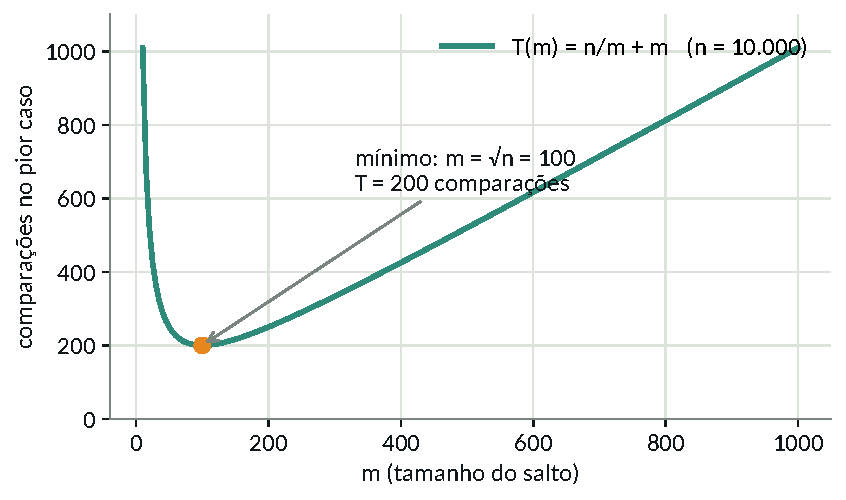
\includegraphics[width=0.72\textwidth]{figuras/f11_busca_saltos.pdf}
  \caption{$T(m)$ para $n = 10.000$: a curva tem um \enquote{vale}. O ponto mais baixo é o melhor
  salto.}
\end{figure}

No ponto mais baixo do vale, a curva fica \enquote{deitada}: a tangente é horizontal, com
inclinação zero. Então basta achar onde $T'(m) = 0$. Escrevendo $\dfrac{n}{m} = n \cdot m^{-1}$ e
usando a regra da potência com $p = -1$:
\[
T'(m) = n \cdot (-1) \cdot m^{-2} + 1 = -\frac{n}{m^2} + 1.
\]
\[
T'(m) = 0 \;\Longleftrightarrow\; \frac{n}{m^2} = 1 \;\Longleftrightarrow\; m^2 = n
\;\Longleftrightarrow\; \boxed{m = \sqrt{n}}.
\]

Com $n = 10.000$: $m = 100$, e o pior caso fica em $T = 100 + 100 = 200$ comparações — contra
10.000 da busca linear. Em geral, $T(\sqrt{n}) = 2\sqrt{n}$: a busca por saltos é $O(\sqrt{n})$.

O programa \codigo{python/busca_saltos.py} testa todos os saltos de 1 a 1.000 e confirma:

\needspace{18\baselineskip}
\lstinputlisting[style=terminal]{tabelas/saida_saltos.txt}

Repare na penúltima linha: vinte valores de $m$, de 91 a 110, empatam em 200. Perto do mínimo,
a curva é quase plana — exatamente o que significa \enquote{inclinação zero}.

\begin{aprofunde}
Como saber que $m = \sqrt{n}$ é um mínimo, e não um máximo? Pela \textbf{segunda derivada}
(a derivada da derivada): $T''(m) = \dfrac{2n}{m^3}$, que é positiva para $m > 0$. Segunda
derivada positiva quer dizer que a inclinação está aumentando: a curva tem a forma de um vale,
e o ponto de inclinação zero é o fundo.
\end{aprofunde}

\section{Comparando crescimentos com limites}

\begin{aprofunde}
Às vezes não é óbvio qual de duas funções cresce mais rápido. Por exemplo: $n \log n$ ou
$n^{1{,}5} = n\sqrt{n}$? Uma técnica é olhar o limite da divisão entre elas quando $n \to \infty$
(capítulo 3): se tende a 0, a de cima cresce mais devagar.

Dividindo as duas por $n$, sobra comparar $\ln n$ com $\sqrt{n}$. As duas vão para o infinito, e
aí entra a \textbf{regra de L'Hôpital}: nesse caso, o limite da divisão é igual ao limite da
divisão das derivadas.
\[
\lim_{n \to \infty} \frac{\ln n}{n^{1/2}}
\;=\; \lim_{n \to \infty} \frac{1/n}{\tfrac{1}{2} n^{-1/2}}
\;=\; \lim_{n \to \infty} \frac{2}{\sqrt{n}} \;=\; 0.
\]
Conclusão: $n \log n$ cresce mais devagar que $n\sqrt{n}$. (Usamos que a derivada de $\ln n$ é
$1/n$.) É por isso que, na hierarquia do capítulo 10, $n \log n$ vem antes de $n^2$, e até
antes de $n^{1{,}5}$.
\end{aprofunde}

\begin{exrapido}
Calcule as derivadas: (a) $n^4$; (b) $5n^2$; (c) $\sqrt{n}$; (d) $\dfrac{1}{n^2}$;
(e) $(n + 1)^2$; (f) $(3n - 2)^2$.
\end{exrapido}

\begin{exrapido}
Na busca por saltos: (a) com $n = 400$, qual é o melhor salto e quantas comparações são feitas
no pior caso? (b) E com $n = 1.000.000$? Compare com a busca linear.
\end{exrapido}

\begin{exrapido}
Um algoritmo faz $T(n) = n^2 + 3n$ passos. Use a derivada para estimar quantos passos a mais ele
faz quando $n$ passa de 100 para 101. Confira calculando $T(101) - T(100)$.
\end{exrapido}

\begin{respostas}
  \resp{11.1} (a) $4n^3$. (b) $10n$. (c) $\dfrac{1}{2\sqrt{n}}$. (d) $n^{-2} \to -2n^{-3} = -\dfrac{2}{n^3}$.
  (e) $2(n + 1)$. (f) $2(3n - 2) \cdot 3 = 18n - 12$.
  \resp{11.2} (a) $m = \sqrt{400} = 20$; $T = 400/20 + 20 = 40$ comparações (contra 400).
  (b) $m = 1.000$; $T = 2.000$ comparações (contra 1.000.000).
  \resp{11.3} $T'(n) = 2n + 3$, então $T'(100) = 203$ passos a mais, aproximadamente. Exato:
  $T(101) - T(100) = (10.201 + 303) - (10.000 + 300) = 204$. A derivada acerta por pouco.
\end{respostas}
